\documentclass[12pt,fleqn]{article}
\usepackage{polyglossia}
\usepackage{fontspec}
\setmainlanguage{serbian}
\newfontfamily\cyrillicfont{PT Sans}[Script=Cyrillic]
\newfontfamily\cyrillicfonttt{PT Sans}[Script=Cyrillic]
\newfontfamily\cyrillicfontsf{PT Sans}[Script=Cyrillic]
\usepackage{authblk}
\usepackage{blindtext}
\usepackage{algorithm}
\usepackage{algpseudocode}
\usepackage{float}
\usepackage{graphicx}
\usepackage[style=numeric,backend=biber]{biblatex}
\addbibresource{literatura.bib}

\title{Проблем ротације усева}
\author{Никола Шутић}
\affil{Математички факултет, Универзитет у Београду}

\begin{document}
\maketitle
\newpage

\tableofcontents
\newpage

\section{Увод}
Традиционално гајењо воће и поврће подразумева вишегодишњу поновљену садњу монокултуре (једне исте биљне врсте) на истом земљишту. Оваква стратегија садње има предност у једноставности планирања и извођења, погодног за механизацију и садње на велико. Међутим, оваква стратегија може изазвати озбиљне проблеме и спречити дугорочну експлоaтацију земље. Проблеми који на овај начин могу да се изазову су, између осталог: исушивање хранљивих супстанци земље, прекомерно размножавање патогена, смањени принос.

С обзиром на напор неких научника и доктора да свет погурају више у смеру здравије исхране и помере од високо обрађене хране, вреди даље истражити и улагати у технике које би помогле и малим газдинствима да произведу веће количине воћа и поврћа за своје потребе.

\section{Проблем ротације усева}
\subsection{Дефиниција проблема}
Уколико на истом земљишту смењујемо биљке које садимо на годишњем, сезонском или неком другом временском интервалу, ми вршимо ротацију усева. Проблемом ротације усева мисли се на његово решење. Решење овог проблема је управо један план садне који описује низ култура и њихових планираних временских интервала за сетву. Описан је концепт ротације усева, али не и шта желимо да добијемо ротацијом. Најчешћи циљ је постизање највећег могућег приноса од одабраних култура. Неки други циљеви који ће бити обрађени у раду су разноврсност или продаја.

\section{Имплементација алгоритма}
\subsection{Генетски алгоритам}
Генетски алгоритам је врста оптимизационог алгоритма чији се рад заснива на генетичким принципма виђеним у природи. Кандидати за решење проблема се називају хромозоми, и они су најчешће дати као математичка репрезентација решења проблема који решавамо. Користећи операторе укрштања и мутације прилагођене проблему, усмеравамо популацију ка бољем прилагођавању захтевима проблема. Као решење проблема управо узимамо најбоље прилагођену јединку из популације.

Сам генетски алгоритам не захтева велико умеће за имплементацију и примену. Највећа тежине ове технике лежи у успешном математичком моделирању проблема, и прилагођавању оператора алгоритма проблему који се решава. У складу с овиме, временом су се издвојили шаблони за моделирање проблема који су се често понављали. У овом раду биће коришћено 0-1 бинарно моделиране проблема.

\subsection{Ротација усева као 0-1 ГА}

У овом одељку ће бити детаљније објашњен приступ моделирања проблема коришћен у овом раду. Ослањајући се на претходни рад \cite{geraldi}, уводе се следеће променљиве које ће бити коришћене:

$x_{ijk} \in \{0,1\}$ - Један ген у плану, вредност обележава да ли је биљка $i$, засађена у периоду $j$, на земљишту $k$.

$N$ - Укупан број биљака узетих у разматрање. Са $n$ ће се обележити ,,празна'' биљка.

$M$ - Број временских периода. Један период узет да буде 15 дана али може бити више или мање по потреби.

$B$ - Скуп скупова биљака одвојених по породицама.

$F$ - Породице биљака.

$I_i$ - Временски периоди за сетву биљке $i$.

$D$ - Скуп биљака које се користе за зелено ђубриво.

\subsection{Мека и тврда ограничења}
За разлику од \cite{geraldi}, ограничења претходно коришћена за потребе програмирања ограничења, овде ће бити имплементиране и коришћене у виду пенала јединке и то: $\sigma_{soft}$ и $\sigma_{hard}$. Огранићења коришћена су:

\begin{minipage}{\textwidth}
\begin{equation}
  \sum_{i=o}^n \sum_{q=0}^{t_i-1} x_{i(j-q)k} \le 1 \qquad j = 1..M,\, k = 1..K
\end{equation}
На истој земљи у једно време може расти само једна биљка.
\end{minipage}

\begin{minipage}{\textwidth}
\begin{equation}
      \sum_{i\in D} \sum_{j\in I_i}x_{ijk} \ge 1 \qquad k = 1..K
    \end{equation}
    Свако земљиште мора бити барем једном ђубрено.
\end{minipage}

\begin{minipage}{\textwidth}
\begin{equation}
      \sum_{j=1}^M x_{njk} \ge 1 \qquad k = 1..K
\end{equation}
Свако земљиште мора имати један период без ичега посађеног.
\end{minipage}

\begin{minipage}{\textwidth}
  \begin{equation} \label{eq:4}
      \sum_{i\in B_f} \sum_{q=0}^{t_i + t_n-1} x_{i(j-q)k} \le  1 \qquad f=1..F,\, j=1..M,\, k=1..K
    \end{equation}
    Ово је управо ограничење ротације усева. На једном земљишту мора бити пауза од једног периода између исте породице биљака.
  \end{minipage}

  Последње ограничење забрањује суседним земљиштима да деле исту породицу биљака у исто време како би се спречило размножавање заједничких патогена и подржала могућа симбиоза између различитих породица.

  \begin{minipage}{\textwidth}
    \begin{equation}
        \sum_{i\in B_f} \sum_{q=0}^{t_i-1} \sum_{a\in A_k} (x_{i(j-q)k} + x_{i(j-q)a}) \le 1 \qquad f = 1..F,\, j = 1..M,\, k = 1..K
      \end{equation}
      $A_k$ коришћено у овој формули представља сва земљишта која су суседна земљишту $k$. Ово ограничење је пенализовано са $\sigma_{soft}$.
\end{minipage}  
  
\subsection{Главна петља}

\begin{minipage}{\textwidth}
Главна петља коришћенa у овом раду је у сагласности са главном петљом генетског алгоритма, дата псеудокодом:
\begin{algorithm}[H]
\caption{Genetic Algorithm}\label{genetic_algo}
\begin{algorithmic}[1]
\State \textbf{Initialize} Population $\leftarrow \{s_1, s_2, \ldots, s_n\}$
\For{$gen\_idx \in \{1, 2, \ldots, numof\_generations\}$}
    \State scores $\leftarrow$ sorted([(fitness(s), s) for s in population])
    \State new\_pop $\leftarrow$ [s[1] for s in scores[:elitism]]
    \For{\_ in range(elitism, population\_size)}
        \State parent\_idx, parent\_idx\_2 $\leftarrow$ rd.choices( range(numof\_parents), k = 2)
        \State parent $\leftarrow$ scores[parent\_idx][1]
        \State parent2 $\leftarrow$ scores[parent\_idx\_2][1]
        \State child $\leftarrow$ parent.crossover(parent2).mutation()
        \State new\_pop.append(child)
    \EndFor
    \State population $\leftarrow$ new\_pop
\EndFor
\end{algorithmic}
\end{algorithm}
\end{minipage}

\subsubsection{Генерисање јединке}
Ослањајући се само на мека и тврда ограничења за усмеравање јединки, показује се да је ово недовољно звог велике димензије проблема, према томе уводи се посебно имплементирано генерисање јединке које води рачуна о ограничењу ротације усева (\ref{eq:4}):


\begin{algorithm}
\caption{Initialize solution}
\begin{algorithmic}[1]
\State \textbf{Function} initialize()
\For {$k = 1$ to $K$}
    \State $plan[:,:,k] \gets generatePlot(k)$
\EndFor
\end{algorithmic}
\end{algorithm}

У функцији $generatePlot$ генеришемо низ садње биљака водећи рачуна о (\ref{eq:4}) тако што мењамо следећу породицу биљака после сваке одабране.

\subsection{Исцрпни алгоритам}
Исрцпни алгоритам за проблем дефинисан на представљени начин је имплементиран у виду генерисања комбинација разматрајући да ли ће се биљка $n$ посадити у времену $t$ на земљишту $k$. С обзиром да простор претраге подлеже комбинаторној експлозији, не може се очекивати добро решење у кратком временском року, што потврђује и тестирање. Најбоље решење нађено оваквом стратегијом подлежући временским ограничењима најчешће прима облик једне биљке (прве или међу првим у претрази) засађене на једном земљишту. Овакво понашање и јесте очекивано имајући у виду изложена ограничења и начин на који су дефинисана. Међутим, у одељку тестирања свакако ће бити приказано решење нађено оваквом стратегијом.

\section{Тестирање и резултати}
Следећи тестови одрађени су са следећим условима: 4 реда земље, сваки ред површине $1m^2$. Редови на вертикалној оси представљају задата земљишта, а јединице на хоризонталној оси представљају временске периоде. Графици који представљају решења су инспирисани аутором \cite{dwave}. Циљна функција коришћена је приказана у наслову графика као и њена вредност за приказан план ротације. С обзиром на разлику генерација и дубине претраге, претпоставка је да се приликом тестирања алгоритми покрећу са истим временским ограничењем.

\subsection{Циљ различитих биљака}
Циљ оптимизације је дат формулом $|N|$ - величина скупа различитих засаћених биљака. Треба подсетити да циљ оптимизације није нужно и фитнес функција, која је у овом раду имплементирана као пенализована циљна функција.

\begin{figure}[H]
  \caption{Исцрпни алгоритам}
  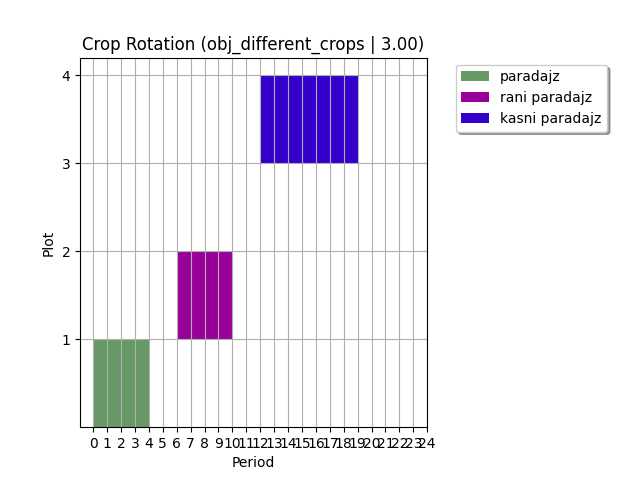
\includegraphics[scale=1]{obj_different_crops_bf}\centering
\end{figure}

\begin{figure}[H]
  \caption{Генетски алгоритам}
  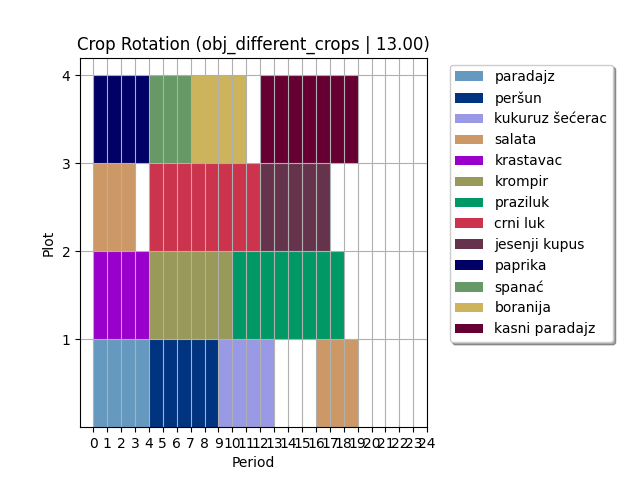
\includegraphics[scale=1]{obj_different_crops_ga}\centering
\end{figure}

\subsection{Циљ највећег приноса}
Циљ оптимизације је дат формулом $\sum x_{ijk} \cdot P_i$, где је $P_i$ теоријски принос биљке $i$. Вредност циљне функције је укупан принос у килограмима (под претпоставком да су спољашњи фактори предвидиви и биљке остваре свој теоријски принос).

\begin{figure}[H]
  \caption{Исцрпни алгоритам - Биљке укључене у овај план су исте као и код претходног циља. Ово није неочекивано имајући у виду да је исцрпна претрага детерминистички алгоритам, и претрага остварује одређени домет за исто предвиђено време.}
  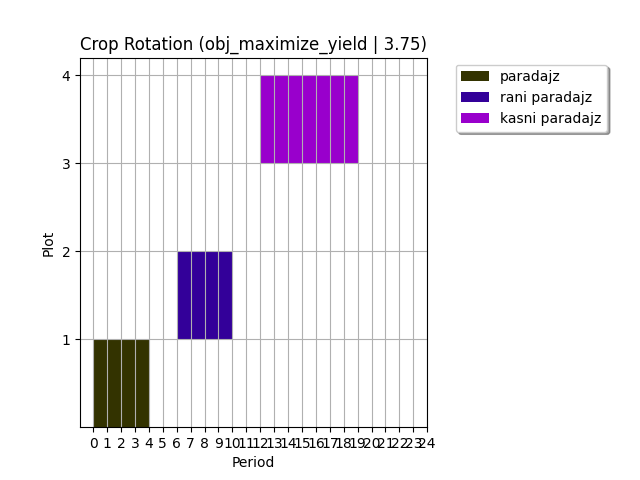
\includegraphics[scale=1]{obj_maximize_yield_bf}\centering

\end{figure}

\begin{figure}[H]
  \caption{Генетски алготирам - Резултат постигнут је теоријски оствариви приход. Ова информација може бити веома корисна у сврху планирања исхране или продаје. Наравно, циљ може бити и укупна зарада од продаје плода.}
  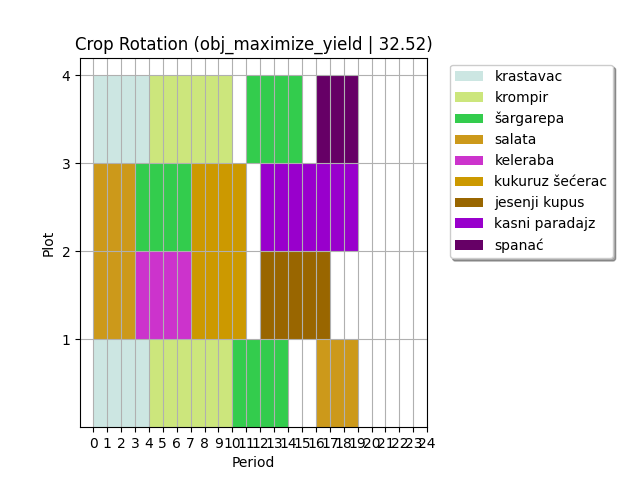
\includegraphics[scale=1]{obj_maximize_yield_ga}\centering
\end{figure}

\section{Закључак}
Занимљиво је приметити да је рад \cite{geraldi} заснован на земљишту у Бразилу, као и радови цитирани у том раду. Ово може бити последица тога што мање развијене земље улажу већи труд у паметније планирање пољопривреде уместо у скупљу и бољу машинерију за обраду.

Такође је вредно истаћи велики недостатак или боље речено недоступност база података које су створене у сврху планирања. У раду је коришћена породица биљака као разлучујући фактор, мада са прецизнијом информацијом (нпр. појединачни захтеви биљака за калијум, фосфор и азот или детаљнија информација о патогенима конкретних биљака) је могуће остварити реалистичније резултате.

Подаци корићшени у овом раду су демонстративне природе и набављени консултацијом са доменским експертом или из каталога семења.

\printbibliography

\end{document}
